% Development

% Main chapter title
%\chapter[toc version]{doc version}
\chapter{Development}

% Short version of the title for the header
%\chaptermark{version for header}

% Chapter Label
% For referencing this chapter elsewhere, use \ref{ChapterTemplate}
\label{Development}

This chapter describes the development of the timetable system, formulating the problem, discussing the implementation of the \ac{mcts} and \ac{hc} hybrid approach, detailing the design choices, algorithmic improvements and integration efforts made throughout the project.

\section{Search Space}

The search space, \(S\),  for this problem is large as it involves a product of all possible event-period-room combinations: \[S = E \cdot P  \cdot R,\] where \(E\) is the set of events, \(P\) is the set of periods (day,timeslot), and \(R\) is the set of rooms.

\section{Problem Formulation}

(...)
The entities in the problem are listed below:

\begin{itemize}
	\item \textbf{Periods, \(P = \{P_1, P_2, ..., P_|_P_|\}\):} Days are divided into fixed timeslots, with periods consisting of a day and a timeslot.

		\unsure[inline]{In the previous work, there is no periods. There are weekdays, a start time and an end time. For now, in the current approach, an event is only associated with a period of one hour and without any link to previous work. If I implement this concept to previous work, an event should be assigned to one or more half-hour periods.}

	\item \textbf{Rooms, \(R = \{R_1, R_2, ..., R_|_R_|\}\):} Each room has a capacity and a type.
		\begin{itemize}
			\item Occupation (the room may be utilized for non-teaching reasons, such as exams) (TODO)
			\item Capacity (number of seats)
			\item Type (TODO)
		\end{itemize}

	\item \textbf{Lecturers, \(L = \{L_1, L_2, ..., L_|_L_|\}\):} 
		\begin{itemize}
			\item Office
			\item Restriction (availability and TODO: preferences for periods)
		\end{itemize}

	\item \textbf{Events, \(E = \{E_1, E_2, ..., E_|_E_|\}\):} Represent the events to be scheduled. Each event has associated attributes:
		\begin{multicols}{2}
		\textbf{Previous work:}
		\begin{itemize}
			\item Start and end time
			\item Weekday
			\item Duration
			\item Lecturer
			\item Room
		\end{itemize}
		\columnbreak
		\textbf{TODO: adicionar ao trabalho anterior?}
		\begin{itemize}
			\item Period
        		\item Capacity (number of students)
        		\item Number of lectures
        		\item Minimum working days (days over which the events of the same block should be spread)
        		\item Available periods
        		\item Priority
		\end{itemize}
		\end{multicols} 

	\item \textbf{Blocks, \(B = \{B_1, B_2, ..., B_|_B_|\}\):} A block may represent a group of related events, such as all events of a subject, or events from the same course and curricular year.
\end{itemize}

\subsection{Constraints}

There are several hard and soft constraints that affect the creation of \ac{fcup} timetables. The following hard and soft constraints were selected, drawing inspiration from those of \ac{itc-2007}:

\textbf{Hard constraints:}

\begin{itemize}
	\item \textbf{H1:} Events belonging to the same subject must be scheduled and must be assigned to distinct periods.
	\item \textbf{H2:} Two events can be scheduled in the same room, but only if they are in different periods.
	\item \textbf{H3:} Events of the same course and curricular year, or taught by the same lecturer, must be scheduled in different periods.
	\item \textbf{TODO H4:} If a room is unavailable in a given period, then no events can be scheduled in that period.
	\item \textbf{H5:} If a lecturer is unavailable in a given period, then no events can be taught by this lecturer in that period.
	\item \textbf{TODO H6:} Lecturers and students must have a free lunch period.
\end{itemize}

\textbf{Soft constraints:}

\begin{itemize}
	\item \textbf{S1:} Events of the same subject should be spread into the given minimum number of days.
	\item \textbf{S2:} Events belonging to the same course and curricular year should be in consecutive periods.
	\item \textbf{S3:} The capacity of the room should be higher or equal than the capacity of the event.
	\item \textbf{S4:} All events of a subject should be given in the same room.
\end{itemize}


%Maximization problem...

\section{Algorithm}

This section describes the key algorithmic components of the system, particularly the hybrid \ac{mcts} with \ac{hc} approach.

\subsection{Monte Carlo Tree Search}

(...)

\subsubsection{\ac{mcts} Tree}

\begin{figure}
      \centering
      \includegraphics[width=0.7\columnwidth]{Development/MCTS_tree.jpg}
      \caption[MCTS tree]
      {MCTS tree}
      \label{fig:mcts_tree}
\end{figure}

Figure \ref{fig:mcts_tree} illustrates the basic structure of the \ac{mcts} tree. The root represents the initial state, where no events have been assigned. The first level corresponds to assigning the first event, \(E1\), to various \(P\) and \(R\). Each child node represents a specific assignment (\((E_1,P_1,R_1),...,(E_1,P_|_P_|,R_|_R_|)\)). Subsequent levels correspond to the sequential assignment of events \(E_2, E_3, ..., E_|_E_|\). Unavailable periods are discarded immediately to reduce the search space.

The events are sorted in advance so that the most difficult event to place is placed first in the tree. The priority of an event (Formula \ref{priority}) is calculated based on:
\begin{itemize}
\item The difference between the number of lectures and minimum working days to prioritize events with more lectures spread over fewer days;
\item The number of available periods, as having more available periods indicates fewer scheduling restrictions;
\item The capacity of an event, which implies that events with greater capacity have higher priority;
\item The number of blocks in which the event is, as events that appear in more blocks are more difficult to allocate.
\end{itemize}

\begin{equation}
  \begin{aligned}
	Priority = (\#lectures - \#min\_working\_days) \cdot 4 \\
	           - \#available\_periods \cdot 3 \\
	          + capacity \cdot 2 \\
	          + \#blocks\label{priority}
  \end{aligned}
\end{equation}

\subsubsection{Tree Nodes}

A node is composed of the following attributes:

\begin{itemize}
\item A \textbf{path} is a dictionary that represents the sequence of actions leading to a node. The root is the only node that has an empty path.

\item A \textbf{parent} is a reference to the parent node, allowing the tree structure to be navigated upwards. The root is the only node that does not have a parent.

\item \textbf{Children} is initialized as an empty list at first but will later hold references to the node's child nodes. 

\item The \textbf{expansion limit} specifies the maximum number of children that a node can have, which helps control the expansion process in the \ac{mcts} algorithm. A value of zero indicates that the node cannot be expanded further.

\item \textbf{Visits} is initialized to 0, tracking the number of times a node has been visited.

\item The \textbf{hard and soft scores} are both initialized to 0, representing the cumulative hard and soft scores for a node, which are used to evaluate the quality of the node's state.

\item The \textbf{best hard and soft penalty results} are initialized to negative infinity, representing the best hard and soft penalty results encountered for a node. These attributes will be updated during the algorithm as better results are found. 
\end{itemize}

\subsubsection{Methodology}

\ref{fig:mcts_steps}(...)

\begin{figure}[H]
      \centering
      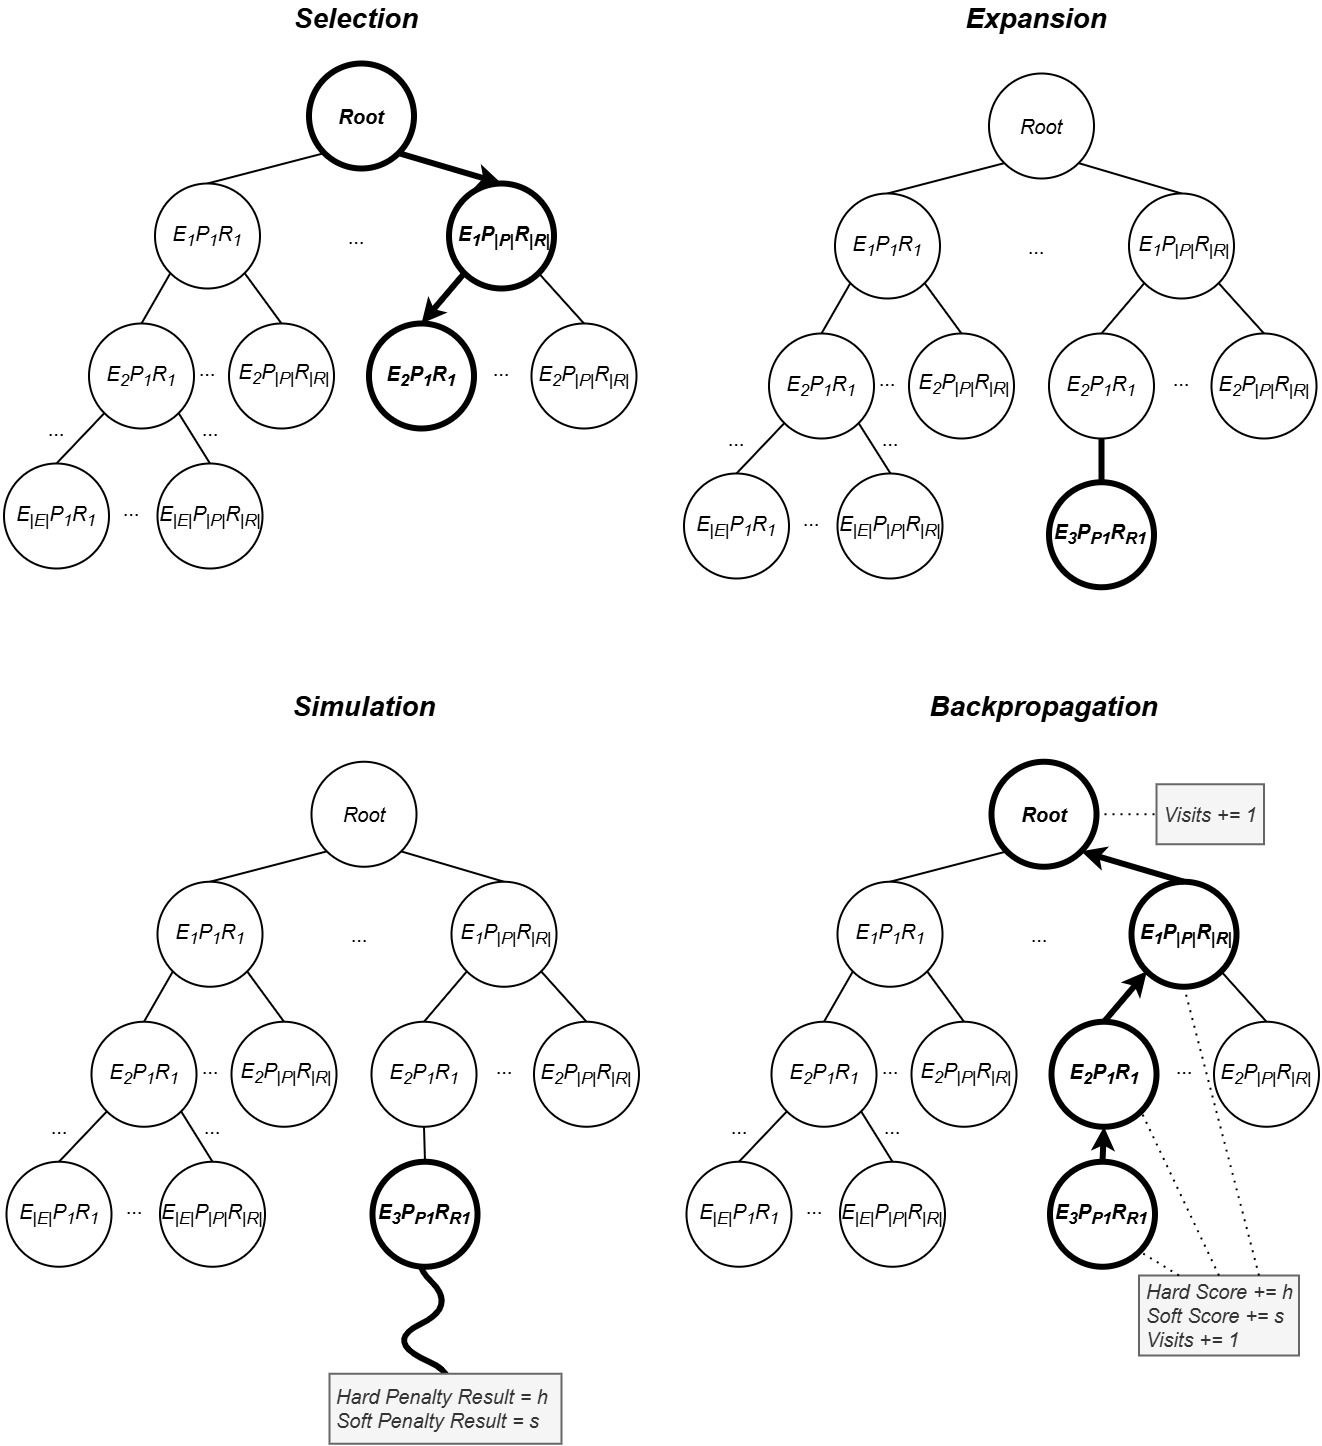
\includegraphics[width=\columnwidth]{Development/MCTS_steps.jpg}
      \caption[MCTS steps]
      {MCTS steps}
      \label{fig:mcts_steps}
\end{figure}

The \(selection\) procedure (Algorithm \ref{selection}) traverses the tree from the root, selecting the best child nodes until reaching a terminal (leaf) node. A node is considered terminal if either it cannot be expanded further (i.e., its \(expansion\_limit\) is 0) or if it has reached the maximum depth (i.e., all the events have been assigned). Conversely, a node is deemed fully expanded if it either has the \(expansion\_limit\) equal to 0 or if the number of its children equals its expansion limit. In the selection process, if a node is not fully expanded, the traversal halts, and that node is selected for further expansion.

The \(best\_child\) function (Algorithm \ref{best_child}) determines the best child node by applying the \ac{uct} formula (\ref{uct_formula}). Initially, it computes the weights for each child node using the hard score. Among the children with the highest hard score, the weights are recalculated based on the soft score. The child node with the highest weight in this second calculation is selected as the best child.

\begin{algorithm}
\caption{Selection}\label{selection}
\begin{algorithmic}[1]
\Procedure{SELECTION()}{}
\State \text{current\_node} $\gets$ \text{root}
\While{\textbf{not} \text{current\_node.}\text{\textit{is\_terminal\_node(len(}events\textit{))}}}
    \If{\textbf{not} \text{current\_node.}\textit{is\_fully\_expanded()}}
    \State \text{break}
    \EndIf
    \State \text{best\_child} $\gets$ \text{current\_node.}\textit{best\_child()}
    \State \text{current\_node} $\gets$ \text{best\_child}
\EndWhile
\State \text{self.current\_node} $\gets$ \text{current\_node}
\EndProcedure
\end{algorithmic}
\end{algorithm}

\begin{algorithm}
\caption{Best Child}\label{best_child}
\begin{algorithmic}[1]
\Function{BEST\_CHILD}{\text{c\_param} = 1.4}
    \State \text{choices\_weights $\gets$ [child.score\_hard $+$ c\_param $\cdot \sqrt{\frac{2 \cdot \log(\text{self.visits})}{\text{child.visits}}}}$
    \text{\textbf{for each} child \textbf{in} self.children]}
    \\
    \State \text{max\_weight $\gets$ max(choices\_weights)}
    \State \text{best\_children $\gets$ [self.children[i] \textbf{for} i, weight \textbf{in} enumerate(choices\_weights) \textbf{if}} \text{weight $==$ max\_weight]}
\\
    \State \text{choices\_weights $\gets$ [child.score\_soft $+$ c\_param $\cdot \sqrt{\frac{2 \cdot \log(\text{self.visits})}{\text{child.visits}}}}$
    \text{\textbf{for each} child \textbf{in} best\_children]}
    \\
    \State \textbf{return} \text{best\_children[choices\_weights.\textit{index(max(}choices\_weights\textit{))}]}
\EndFunction
\end{algorithmic}
\end{algorithm}

The \(expansion\) procedure (Algorithm \ref{expansion}) is responsible for expanding the node previously selected, \(current\_node\), by adding a new child node. It starts by retrieving the next unvisited event based on the current node's depth, which is the length of its path.

If the event has available periods, the algorithm retrieves the corresponding weekday and timeslot. Next, the \(find\_available\_rooms\) function (Algorithm \ref{find_available_rooms}) finds the available rooms per period for the event, removing rooms that are occupied by other events and filtering rooms based on their capacity. If there are available rooms, it selects a room and creates a new event with the selected room, weekday, and timeslot.

The procedure then calculates the expansion limit for the next event in the timetable, i.e., the number of children that the new current node child can have. If no more events remain, the limit is set to zero. Otherwise, it sums the number of available rooms per period for the next event.
 
Finally, a new child node is created and added to the tree. The current node is updated to this newly created node.

\begin{algorithm}
\caption{Expansion (simplified)}\label{expansion}
\begin{algorithmic}[1]
\Procedure{EXPANSION()}{}
    \State \text{event} $\gets$ \text{events[current\_node.\textit{depth()}]}
    \State \text{available\_periods} $\gets$ \text{event["Available\_Periods"]}
	\\
    \State \text{period} $\gets$ \text{\textit{len(}current\_node.children\textit{)}}
    \State \text{period\_index} $\gets$ \text{period} \% \text{\textit{len(}available\_periods\textit{)}}
    \State \text{new\_weekday, new\_timeslot} $\gets$ \text{available\_periods[period\_index]}
    \\
    \State \text{available\_rooms} $\gets$ \textit{find\_available\_rooms()}
    \State \text{new\_room\_index} $\gets$ \text{period} // \text{\textit{len(}available\_periods\textit{)}} \% \text{\textit{len(}available\_rooms\textit{)}}
    \State \text{new\_room} $\gets$ \text{available\_rooms[new\_room\_index]}
    \\
   \State \text{new\_event $\gets$ \{**event, "RoomId:new\_room, "WeekDay":new\_weekday, "Timeslot":new\_timeslot\}}
   \State \text{next\_event} $\gets$ \text{events[current\_node.\textit{depth()} + 1] \textbf{if} current\_node.\textit{depth()} + 1 $<$ \textit{len(}events\textit{)}}} \textbf{else} \texttt{None}

    \\
\If{\text{next\_event} \textbf{is} \texttt{None}}
    \State \text{expansion\_limit} $\gets 0$ 
\Else
	\State \text{expansion\_limit} $\gets$ \text{\textit{sum(len(}rooms\textit{)} \textbf{for} rooms \textbf{in} \textit{find\_available\_rooms()}\textit{)}}}
\EndIf
        \\
    \State \text{child\_node} $\gets$ \text{MCTSNode(expansion\_limit=expansion\_limit, parent=current\_node,} \text{path=current\_node.path+[new\_event])}
    \State \text{child\_node.path} $\gets$ \text{current\_node.path} + [\text{new\_event}]
    \State \text{current\_node.children.\textit{append(}child\_node\textit{)}}
    \State \text{current\_node} $\gets$ \text{child\_node}
\EndProcedure
\end{algorithmic}
\end{algorithm}

\begin{algorithm}
\caption{Find Available Rooms}\label{find_available_rooms}
\begin{algorithmic}[1]
\Function{find\_available\_rooms}{event\_capacity, rooms, events, available\_periods}
    \State \text{period\_room\_availability} $\gets$ \{\text{period: \{room["Id"] \textbf{for} room \textbf{in} rooms\}} \textbf{for} period \textbf{in} available\_periods\}
    \\
    \For{\text{other\_event \textbf{in} events}}
        \State \text{occupied\_period} $\gets$ \text{(other\_event["WeekDay"], other\_event["Timeslot"])}
        \If{\text{occupied\_period \textbf{in} period\_room\_availability}}
            \State \text{period\_room\_availability[occupied\_period].\textit{discard(}other\_event["RoomId"]\textit{)}}
        \EndIf
    \EndFor
    \\
    \State \text{suitable\_rooms} $\gets$ \text{\{room["Id"] \textbf{for} room \textbf{in} rooms \textbf{if} room["Capacity"] $>=$ event\_capacity\}}
    \\
    \For{\text{period \textbf{in} available\_periods}}
        \If{\text{period\_room\_availability[period]}}
            \State \text{period\_room\_availability[period] $\gets$ period\_room\_availability[period] $\cap$ suitable\_rooms} 
            \textbf{if} \text{period\_room\_availability[period] $\cap$ suitable\_rooms \textbf{else} period\_room\_availability[period]}
        \EndIf
    \EndFor
    \\
    \State \Return \text{period\_room\_availability}
\EndFunction
\end{algorithmic}
\end{algorithm}

The simulation phase estimates the value of multiple actions, in this case, distinct event allocations, which will guide the selection and expansion steps in future iterations. 

A random event allocation approach was initially explored but produced suboptimal results. Thus, a more structured method was implemented.

Therefore, the \(simulation\) function starts to create a copy of the current node's path and adds and sorts all the remaining events (events not yet allocated). They are sorted based on whether they are in the \(unassigned\_events\) list, which are the events not scheduled in the previous simulated timetables, and then based on their priority. This ensures that higher-priority events are scheduled first.

For each unvisited event in the timetable, the \(find\_best\_room\_and\_period\) helper function finds the best available period and room combination. The approach is similar to constraint programming as it iterates through all the available periods and rooms, calculating the hard and soft penalties for each combination. The combination with no hard penalties and with the lowest soft penalty is selected as the best option. If more than one combination is found under those conditions, one of them is chosen randomly. The event is then updated with the selected room, weekday, and timeslot. If no suitable room and period are found, the event is added to the list of \(unassigned\_events\).

After scheduling all events, the \(evaluate\_timetable\) function calculates the result of the simulation, i.e., the hard and soft penalties of the simulated timetable.

The \(update\_penalties\) procedure is then called to update the best and worst penalty score based on the simulation results. If a new best result is found, the timetable is saved to a file. If a new best result is found and the hard penalty is zero, indicating a feasible solution, the Hill Climbing Algorithm (section \ref{hill_climbing_section}) is used to further optimize the timetable.

The normalization formula \ref{normalization_formula} \cite{pedroso_tree_2015} is applied to standardize the simulation results:

\begin{equation}
X(n) = \frac{e^a - 1}{e - 1}, \quad \text{with } a = \frac{\hat{w}^* - \hat{z}_n^*}{\hat{w}^* - \hat{z}^*},\label{normalization_formula}
\end{equation}
where \(\hat{z}^*\) and \(\hat{w}^*\) represent the best and the worst simulation results in the entire tree, and \(\hat{z}_n^*\) is the best simulation result under node \(n\).

\begin{algorithm}
\caption{Simulation (simplified)}\label{simulation}
\begin{algorithmic}[1]
\Function{SIMULATION}{}
    \State \text{simulated\_timetable} $\gets$ \text{copy(current\_node.path)}
    \State \text{simulated\_timetable[self.current\_node.depth():] $\gets$ sorted(events[current\_node.depth():],} \text{key=lambda event: (event["Id"] \textbf{in}} \text{unassigned\_events, event["Priority"], random()), reverse=True)}
\\
    \For{\text{i, event} \textbf{in} \text{enumerate(remaining\_events)}}
        \State \text{best\_room\_and\_period} $\gets$ \textit{find\_best\_room\_and\_period()}
        \If{\text{best\_room\_and\_period} \textbf{exists}}
            \State \text{room, weekday, timeslot} $\gets$ \text{best\_room\_and\_period}
            \State \text{update\_event()}
        \ElsIf{\text{event["Id"]} \textbf{not in} \text{unassigned\_events}}
            \State \text{unassigned\_events.append(event["Id"])}
        \EndIf
    \EndFor
\\
    \State \text{hard\_penalty\_result, soft\_penalty\_result} $\gets$ \text{\textit{evaluate\_timetable(}simulated\_timetable\textit{)}}
    \State \text{\textit{update\_penalties}(hard\_penalty\_result, soft\_penalty\_result\textit{)}}
\\
    \If{\text{hard\_penalty\_result $>$ best\_result\_hard} \textbf{or} 
         (\text{hard\_penalty\_result $==$ best\_result\_hard} \textbf{and} 
         \text{soft\_penalty\_result} $>$ \text{best\_result\_soft})}
        \State \text{best\_result\_hard} $\gets$ \text{hard\_penalty\_result}
        \State \text{best\_result\_soft} $\gets$ \text{soft\_penalty\_result}
        \State \textbf{with} \text{\textit{open(}output\_filename, 'w'\textit{)}} \textbf{as} \textit{file}:
        \State \hskip1em \textit{write\_best\_simulation\_result\_to\_file()}
	 \If{\text{hard\_'penalty\_result} $==$ \text{0}}
		\State \text{simulated\_timetable, best\_result\_hard, best\_result\_soft = hill\_climber.\textit{run\_hill\_climbing()}}
             \State \text{\textit{update\_penalties}(best\_result\_hard, best\_result\_soft\textit{)}}
       \EndIf
    \EndIf
\\
    \State \text{simulation\_result\_hard} $\gets$ \text{\textit{normalize\_hard(}current\_node.best\_hard\_penalty\_result\textit{)}}
    \State \text{simulation\_result\_soft} $\gets$ \text{\textit{normalize\_soft(}current\_node.best\_soft\_penalty\_result\textit{)}}
\\
    \State \Return \text{simulation\_result\_hard, simulation\_result\_soft}
\EndFunction
\end{algorithmic}
\end{algorithm}

The \(backpropagation\) procedure (Algorithm \ref{backpropagation}) updates the tree based on the simulation results. 

It starts from the current node, which is the leaf node where the simulation occurred, and moves up until reaching the root node. During this process, it performs updates for each node in the path, including incrementing the number of visits and updating the hard and soft scores with the simulation results. 

\begin{algorithm}
\caption{Backpropagation}\label{backpropagation}
\begin{algorithmic}[1]
\Procedure{BACKPROPAGATION}{\text{simulation\_result\_hard}, \text{simulation\_result\_soft}}
    \State \text{node} $\gets$ \text{current\_node}
    \While{\text{node} \textbf{is not} \texttt{None}}
        \State \text{node.visits} $\gets$ \text{node.visits} $+ 1$
        \State \text{node.score\_hard} $\gets$ \text{node.score\_hard} $+$ \text{simulation\_result\_hard}
        \State \text{node.score\_soft} $\gets$ \text{node.score\_soft} $+$ \text{simulation\_result\_soft}
        \State \text{node} $\gets$ \text{node.parent}
    \EndWhile
\EndProcedure
\end{algorithmic}
\end{algorithm}

\subsection{Hill climbing}\label{hill_climbing_section}

The \ac{hc} algorithm is applied as a local search method to further optimize the timetable obtained from the \ac{mcts} simulation phase. After finding a feasible solution with \ac{mcts}, \ac{HC} refines the solution by exploring neighboring states. 
(...)

\subsection{Frontend}

The development process involved several adaptations and refinements. Initially, the previous work was analyzed and made functional, serving as a baseline for the new system. The \ac{mcts} algorithm was being developed while also being integrated into the frontend. However, as the focus shifted towards adapting it to the \ac{itc-2007} track 3 benchmark for performance evaluation and fine-tuning the algorithm, the frontend development gradually took a backseat. Over time, the algorithm evolved significantly, diverging from its original form, which made it challenging to align with the prior work.

%\begin{figure}
%    \centering
%      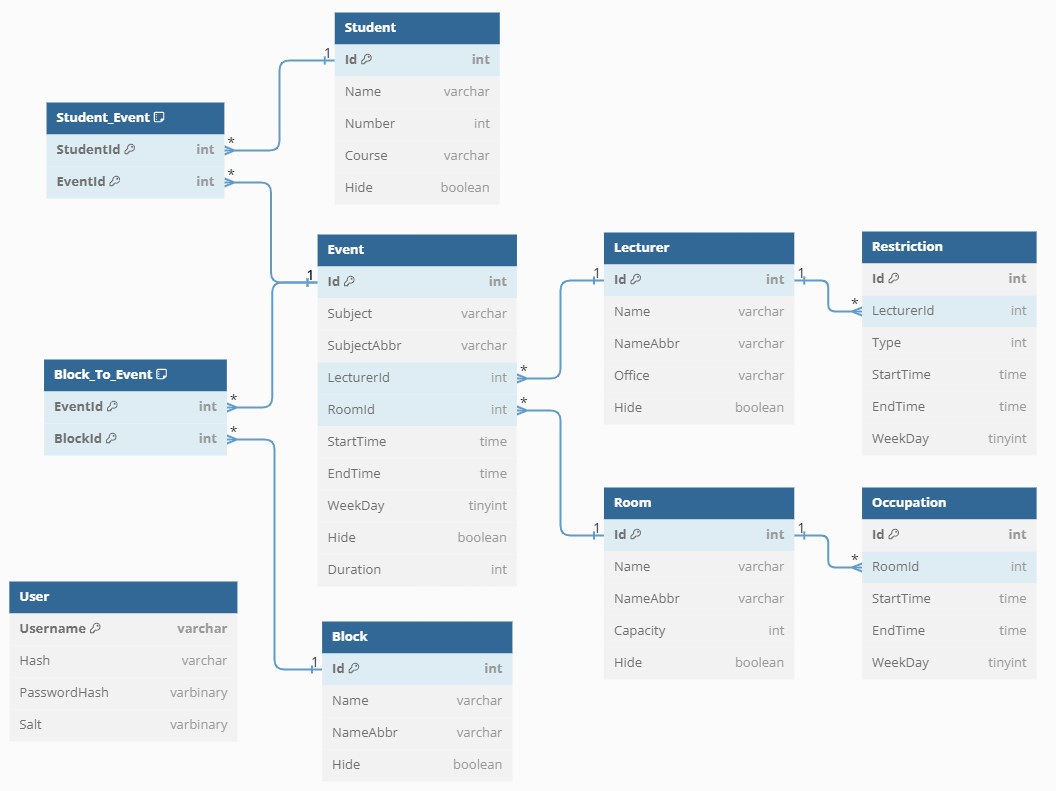
\includegraphics[width=1.1\columnwidth]{Development/uml.png}
%      \caption[UML]
%      {UML}
%      \label{fig:uml}
%\end{figure}